
%%--------------------------------------------------
%% Halliday: Fundamentals of Physics
%%--------------------------------------------------


%% Chapter 03: Vectors
%%--------------------------------------------------


%% Learning Objectives
%%--------------------------------------------------

%% 3.01: Add vectors by drawing them in head-to-tail arrangements, applying the commutative and associative laws.
%% 3.02: Subtract a vector from a second one.
%% 3.03: Calculate the components of a vector on a given coordinate system, showing them in a drawing.
%% 3.04: Given the components of a vector, draw the vector and determine its magnitude and orientation.
%% 3.05: Convert angle measures between degrees and radians.


%% Halliday Multiple Choice Questions
%%--------------------------------------------------
\element{halliday-mc}{
\begin{question}{halliday-ch03-q01}
    We say that the displacement of a particle is a vector quantity.
    Our best justification for this assertion is:
    \begin{choices}
        \wrongchoice{displacement can be specified by a magnitude and a direction}
      \correctchoice{operating with displacements according to the rules for manipulating vectors leads to results in agreement with experiments}
        \wrongchoice{a displacement is obviously not a scalar}
        \wrongchoice{displacement can be specified by three numbers}
        \wrongchoice{displacement is associated with motion}
    \end{choices}
\end{question}
}

\element{halliday-mc}{
\begin{question}{halliday-ch03-q02}
    The vectors $\vec{a}$, $\vec{b}$, and $\vec{c}$ are related by $\vec{c}=\vec{b}-\vec{a}$.
    Which diagram below illustrates this relationship?
    \begin{multicols}{2}
    \begin{choices}[o]
        \AMCboxDimensions{down=-1.0cm}
        \wrongchoice{
            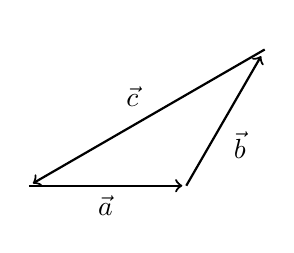
\begin{tikzpicture}
                \draw[white] (0,-1em) rectangle (3.00,2.00);
                \draw[thick,->] (0,0) -- (0:1.95) node[pos=0.5,anchor=north] {$\vec{a}$};
                \draw[thick,->] (0:2) -- ++(60:1.9) node[pos=0.5,anchor=north west] {$\vec{b}$};
                \draw[thick,->] (30:3.46) -- ++(210:3.4) node[pos=0.5,anchor=south east] {$\vec{c}$};
            \end{tikzpicture}
        }
        \wrongchoice{
            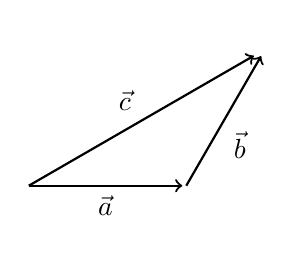
\begin{tikzpicture}
                \draw[white] (0,-1em) rectangle (3.00,2.00);
                \draw[thick,->] (0,0) -- (0:1.95) node[pos=0.5,anchor=north] {$\vec{a}$};
                \draw[thick,->] (0:2) -- ++(60:1.9) node[pos=0.5,anchor=north west] {$\vec{b}$};
                \draw[thick,->] (0:0) -- ++(30:3.30) node[pos=0.5,anchor=south east] {$\vec{c}$};
            \end{tikzpicture}
        }
        \wrongchoice{
            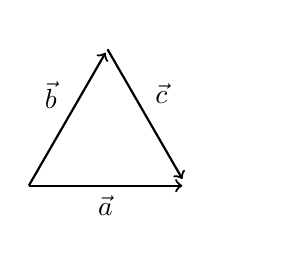
\begin{tikzpicture}
                \draw[white] (0,-1em) rectangle (3.00,2.00);
                \draw[thick,->] (0,0) -- (0:1.95) node[pos=0.5,anchor=north] {$\vec{a}$};
                \draw[thick,->] (0,0) -- (60:1.95) node[pos=0.5,anchor=south east] {$\vec{b}$};
                \draw[thick,->] (60:2) -- ++ (-60:1.9) node[pos=0.5,anchor=south west] {$\vec{c}$};
            \end{tikzpicture}
        }
        %% ANS is D
        \correctchoice{
            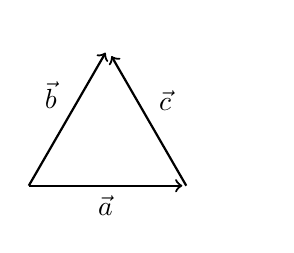
\begin{tikzpicture}
                \draw[white] (0,-1em) rectangle (3.00,2.00);
                \draw[thick,->] (0,0) -- (0:1.95) node[pos=0.5,anchor=north] {$\vec{a}$};
                \draw[thick,->] (0,0) -- (60:1.95) node[pos=0.5,anchor=south east] {$\vec{b}$};
                \draw[thick,->] (0:2) -- ++(120:1.9) node[pos=0.5,anchor=south west] {$\vec{c}$};
            \end{tikzpicture}
        }
        \wrongchoice{
            
\begin{tikzpicture}
                \draw[white] (0,-1em) rectangle (3.00,2.00);
                \node[anchor=center,text width=2cm] at (1.0,0.75) {None of the provided};
            \end{tikzpicture}
        }
    \end{choices}
    \end{multicols}
\end{question}
}

\element{halliday-mc}{
\begin{question}{halliday-ch03-q03}
    A vector of magnitude 3 \emph{cannot} be added to a vector of magnitude 4 so that the magnitude of the resultant is:
    \begin{multicols}{3}
    \begin{choices}
      \correctchoice{zero}
        \wrongchoice{1}
        \wrongchoice{3}
        \wrongchoice{5}
        \wrongchoice{7}
    \end{choices}
    \end{multicols}
\end{question}
}

\element{halliday-mc}{
\begin{question}{halliday-ch03-q04}
    A vector of magnitude 20 is added to a vector of magnitude 25.
    The magnitude of this sum might be:
    \begin{multicols}{3}
    \begin{choices}
        \wrongchoice{zero}
        \wrongchoice{3}
      \correctchoice{12}
        \wrongchoice{47}
        \wrongchoice{50}
    \end{choices}
    \end{multicols}
\end{question}
}

\element{halliday-mc}{
\begin{question}{halliday-ch03-q05}
    A vector $\vec{S}$ of magnitude 6 and another vector $\vec{T}$ have a sum of magnitude 12.
    The vector $\vec{T}$:
    \begin{choices}
      \correctchoice{must have a magnitude of at least 6 but no more than 18}
        \wrongchoice{may have a magnitude of 20}
        \wrongchoice{cannot have a magnitude greater than 12}
        \wrongchoice{must be perpendicular to S}
        \wrongchoice{must be perpendicular to the vector sum}
    \end{choices}
\end{question}
}

\element{halliday-mc}{
\begin{question}{halliday-ch03-q06}
    The vector $-\vec{A}$ is:
    \begin{choices}
        \wrongchoice{greater than $\vec{A}$ in magnitude}
        \wrongchoice{less than $\vec{A}$ in magnitude}
        \wrongchoice{in the same direction as $\vec{A}$}
      \correctchoice{in the direction opposite to $\vec{A}$}
        \wrongchoice{perpendicular to $\vec{A}$}
    \end{choices}
\end{question}
}

\element{halliday-mc}{
\begin{question}{halliday-ch03-q07}
    The vector $\vec{V}_3$ in the diagram is equal to:
    \begin{center}
    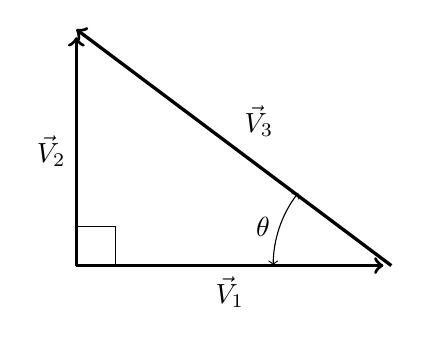
\begin{tikzpicture}
        %% Vectors
        \draw[very thick,->] (0,0) -- ++(0:3.9) node[pos=0.5,anchor=north] {$\vec{V}_1$};
        \draw[very thick,->] (0,0) -- ++(90:2.9) node[pos=0.5,anchor=east] {$\vec{V}_2$};
        \draw[very thick,->] (4,0) -- (0,3) node[pos=0.5,anchor=south west] {$\vec{V}_3$};
        %% Angles
        \draw[<->] (2.5,0) arc (180:142:1.5) node[pos=0.5,anchor=east] {$\theta$};
        \draw (0.5,0.0) -- (0.5,0.5) -- (0.0,0.5);
    \end{tikzpicture}
    \end{center}
    \begin{multicols}{2}
    \begin{choices}
        \wrongchoice{$\vec{V}_1 - \vec{V}_2$}
        \wrongchoice{$\vec{V}_1 + \vec{V}_2$}
      \correctchoice{$\vec{V}_2 - \vec{V}_1$}
        \wrongchoice{$\vec{V}_1 \cos\theta$}
        \wrongchoice{$\dfrac{\vec{V}_1}{\cos\theta}$}
    \end{choices}
    \end{multicols}
\end{question}
}

\element{halliday-mc}{
\begin{question}{halliday-ch03-q08}
    If $\left|\vec{A} + \vec{B}\right|^2 = A^2 + B^2$, then:
    \begin{choices}
         \wrongchoice{$A$ and $B$ must be parallel and in the same direction}
         \wrongchoice{$A$ and $B$ must be parallel and in opposite directions}
         \wrongchoice{either $A$ or $B$ must be zero}
         \wrongchoice{the angle between $A$ and $B$ must be \ang{60}}
       \correctchoice{none of the provided are true}
    \end{choices}
\end{question}
}

\element{halliday-mc}{
\begin{question}{halliday-ch03-q09}
    If $\left|\vec{A} + \vec{B}\right| = A + B$ and neither $\vec{A}$ nor $\vec{B}$ vanish,
        then:
    \begin{choices}
      \correctchoice{$A$ and $B$ are parallel and in the same direction}
        \wrongchoice{$A$ and $B$ are parallel and in opposite directions}
        \wrongchoice{the angle between $A$ and $B$ is \ang{45}}
        \wrongchoice{the angle between $A$ and $B$ is \ang{60}}
        \wrongchoice{$A$ is perpendicular to $B$}
    \end{choices}
\end{question}
}

\element{halliday-mc}{
\begin{question}{halliday-ch03-q10}
    If $\left|\vec{A} - \vec{B}\right| = A + B$ and neither $A$ nor $B$ vanish,
        then:
    \begin{choices}
        \wrongchoice{$A$ and $B$ are parallel and in the same direction}
      \correctchoice{$A$ and $B$ are parallel and in opposite directions}
        \wrongchoice{the angle between $A$ and $B$ is \ang{45}}
        \wrongchoice{the angle between $A$ and $B$ is \ang{60}}
        \wrongchoice{$A$ is perpendicular to $B$}
    \end{choices}
\end{question}
}

\element{halliday-mc}{
\begin{question}{halliday-ch03-q11}
    Four vectors ($\vec{A}$, $\vec{B}$, $\vec{C}$, $\vec{D}$) all have the same magnitude.
    The angle $\theta$ between adjacent vectors is \ang{45} as shown.
    \begin{center}
    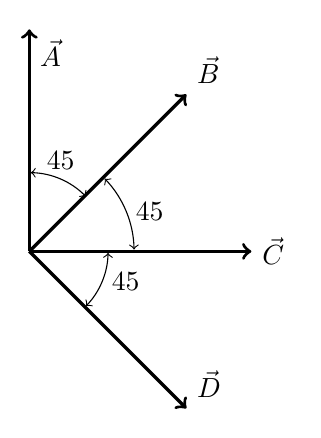
\begin{tikzpicture}
        %% Vectors
        \draw[very thick,->] (0,0) -- ++(90:2.82) node[pos=1.0,anchor=north west] {$\vec{A}$};
        \draw[very thick,->] (0,0) -- ++(45:2.82) node[pos=1.0,anchor=south west] {$\vec{B}$};
        \draw[very thick,->] (0,0) -- ++(0:2.82) node[pos=1.0,anchor=west] {$\vec{C}$};
        \draw[very thick,->] (0,0) -- ++(-45:2.82) node[pos=1.0,anchor=south west] {$\vec{D}$};
        %% Angles
        \draw[<->] (44:1) arc (44:89:1) node[pos=0.5,anchor=south] {\ang{45}};
        \draw[<->] (1:1.33) arc (1:44:1.33) node[pos=0.5,anchor=west] {\ang{45}};
        \draw[<->] (-1:1) arc (-1:-44:1) node[pos=0.5,anchor=west] {\ang{45}};
    \end{tikzpicture}
    \end{center}
    The correct vector equation is:
    \begin{choices}
        \wrongchoice{$\vec{A} - \vec{B} - \vec{C} + \vec{D} = 0$}
      \correctchoice{$\vec{B} + \vec{D} - \sqrt{2}\vec{C} = 0$}
        \wrongchoice{$\vec{A} + \vec{B} = \vec{B} + \vec{D}$}
        \wrongchoice{$\vec{A} + \vec{B} + \vec{C} + \vec{D} = 0$}
        \wrongchoice{$\dfrac{\vec{A} + \vec{C}}{\sqrt{2}} = -\vec{B}$}
    \end{choices}
\end{question}
}

\element{halliday-mc}{
\begin{question}{halliday-ch03-q12}
    Vectors $A$ and $B$ lie in the $xy$ plane.
    We can deduce that $A=B$ if:
    \begin{choices}
        \wrongchoice{$A_x^2 + A_y^2 = B_x^2 + B_y^2$}
        \wrongchoice{$A_x + A_y = B_x + B_y$}
      \correctchoice{$A_x = B_x$ and $A_y = B_y$}
        \wrongchoice{$\dfrac{A_y}{A_x} = \dfrac{B_y}{B_x}$}
        \wrongchoice{$A_x = A_y$ and $B_x = B_y$}
    \end{choices}
\end{question}
}

\element{halliday-mc}{
\begin{question}{halliday-ch03-q13}
    A vector has a magnitude of 12.
    When its tail is at the origin it lies between the positive $x$ axis and the negative $y$ axis and makes an angle of \ang{30} with the $x$ axis.
    Its $y$ component is:
    \begin{multicols}{3}
    \begin{choices}
        \wrongchoice{$\dfrac{6}{\sqrt{3}}$}
        \wrongchoice{$-6\sqrt{3}$}
        \wrongchoice{$6$}
      \correctchoice{$-6$}
        \wrongchoice{$12$}
    \end{choices}
    \end{multicols}
\end{question}
}

\element{halliday-mc}{
\begin{question}{halliday-ch03-q14}
    If the $x$ component of a vector $\vec{A}$,
        in the $xy$ plane, is half as large as the magnitude of the vector,
        the tangent of the angle between the vector and the $x$ axis is:
    \begin{multicols}{3}
    \begin{choices}
        \wrongchoice{$\sqrt{3}$}
        \wrongchoice{$\dfrac{1}{2}$}
        \wrongchoice{$\sqrt{\dfrac{3}{2}}$}
      \correctchoice{$\dfrac{3}{2}$}
        \wrongchoice{$3$}
    \end{choices}
    \end{multicols}
\end{question}
}

\element{halliday-mc}{
\begin{question}{halliday-ch03-q15}
    If ${\vec{A} = \left(\SI{6}{\meter}\right)\hat{\imath} - \left(\SI{8}{\meter}\right)\hat{\jmath}}$ then $4\vec{A}$ has magnitude:
    \begin{multicols}{3}
    \begin{choices}
        \wrongchoice{\SI{10}{\meter}}
        \wrongchoice{\SI{20}{\meter}}
        \wrongchoice{\SI{30}{\meter}}
      \correctchoice{\SI{40}{\meter}}
        \wrongchoice{\SI{50}{\meter}}
    \end{choices}
    \end{multicols}
\end{question}
}

\element{halliday-mc}{
\begin{question}{halliday-ch03-q16}
    A vector has a component of \SI{10}{\meter} in the $+x$ direction,
        a component of \SI{10}{\meter} in the $+y$ direction,
        and a component of \SI{5}{\meter} in the $+z$ direction.
    The magnitude of this vector is:
    \begin{multicols}{3}
    \begin{choices}
        \wrongchoice{zero}
      \correctchoice{\SI{15}{\meter}}
        \wrongchoice{\SI{20}{\meter}}
        \wrongchoice{\SI{25}{\meter}}
        \wrongchoice{\SI{225}{\meter}}
    \end{choices}
    \end{multicols}
\end{question}
}

\element{halliday-mc}{
\begin{question}{halliday-ch03-q17}
    Let $\vec{V} = \left(\SI{2.00}{\meter}\right)\hat{\imath} + \left(\SI{6.00}{\meter}\right)\hat{\jmath} - \left(\SI{3.00}{\meter}\right)\hat{k}$.
    The magnitude of $\vec{V}$ is:
    \begin{multicols}{3}
    \begin{choices}
        \wrongchoice{\SI{5.00}{\meter}}
        \wrongchoice{\SI{5.57}{\meter}}
      \correctchoice{\SI{7.00}{\meter}}
        \wrongchoice{\SI{7.42}{\meter}}
        \wrongchoice{\SI{8.54}{\meter}}
    \end{choices}
    \end{multicols}
\end{question}
}

\element{halliday-mc}{
\begin{question}{halliday-ch03-q18}
    A vector in the $xy$ plane has a magnitude of \SI{25}{\meter} and an $x$ component of \SI{12}{\meter}.
    The angle it makes with the positive $x$ axis is:
    \begin{multicols}{3}
    \begin{choices}
        \wrongchoice{\ang{26}}
        \wrongchoice{\ang{29}}
      \correctchoice{\ang{61}}
        \wrongchoice{\ang{64}}
        \wrongchoice{\ang{241}}
    \end{choices}
    \end{multicols}
\end{question}
}

\element{halliday-mc}{
\begin{question}{halliday-ch03-q19}
    The angle between $A=\left(\SI{25}{\meter}\right)\hat{\imath} + \left(\SI{45}{\meter}\right)\hat{\jmath}$ and the positive $x$ axis is:
    \begin{multicols}{3}
    \begin{choices}
        \wrongchoice{\ang{29}}
      \correctchoice{\ang{61}}
        \wrongchoice{\ang{151}}
        \wrongchoice{\ang{209}}
        \wrongchoice{\ang{241}}
    \end{choices}
    \end{multicols}
\end{question}
}

\element{halliday-mc}{
\begin{question}{halliday-ch03-q20}
    The angle between $\vec{A} = \left(\SI{-25}{\meter}\right)\hat{\imath} + \left(\SI{45}{\meter}\right)\hat{\jmath}$ and the positive $x$ axis is:
    \begin{multicols}{3}
    \begin{choices}
        \wrongchoice{\ang{29}}
        \wrongchoice{\ang{61}}
      \correctchoice{\ang{119}}
        \wrongchoice{\ang{151}}
        \wrongchoice{\ang{209}}
    \end{choices}
    \end{multicols}
\end{question}
}

\element{halliday-mc}{
\begin{question}{halliday-ch03-q21}
    Let $\vec{A} = \left(\SI{2}{\meter}\right)\hat{\imath} + \left(\SI{6}{\meter}\right)\hat{\jmath} - \left(\SI{3}{\meter}\right)\hat{k}$
        and $\vec{B} = \left(\SI{4}{\meter}\right)\hat{\imath} + \left(\SI{2}{\meter}\right)\hat{\jmath} + \left(\SI{1}{\meter}\right)\hat{k}$.
    The vector sum $\vec{S} = \vec{A}+\vec{B}$ is:
    \begin{choices}
      \correctchoice{$\left(\SI{6}{\meter}\right)\hat{\imath} + \left(\SI{8}{\meter}\right)\hat{\jmath} - \left(\SI{2}{\meter}\right)\hat{k}$}
        \wrongchoice{$\left(\SI{-2}{\meter}\right)\hat{\imath} + \left(\SI{4}{\meter}\right)\hat{\jmath} - \left(\SI{4}{\meter}\right)\hat{k}$}
        \wrongchoice{$\left(\SI{2}{\meter}\right)\hat{\imath} − \left(\SI{4}{\meter}\right)\hat{\jmath} + \left(\SI{4}{\meter}\right)\hat{k}$}
        \wrongchoice{$\left(\SI{8}{\meter}\right)\hat{\imath} + \left(\SI{12}{\meter}\right)\hat{\jmath} - \left(\SI{3}{\meter}\right)\hat{k}$}
        \wrongchoice{none of the provided}
    \end{choices}
\end{question}
}

\element{halliday-mc}{
\begin{question}{halliday-ch03-q22}
    Let $\vec{A} = \left(\SI{2}{\meter}\right)\hat{\imath} + \left(\SI{6}{\meter}\right)\hat{\jmath} - \left(\SI{3}{\meter}\right)\hat{k}$
        and $\vec{B} = \left(\SI{4}{\meter}\right)\hat{\imath} + \left(\SI{2}{\meter}\right)\hat{\jmath} + \left(\SI{1}{\meter}\right)\hat{k}$.
    The vector difference $\vec{D} = \vec{A} - \vec{B}$ is:
    \begin{choices}
        \wrongchoice{$\left(\SI{6}{\meter}\right)\hat{\imath} + \left(\SI{8}{\meter}\right)\hat{\jmath} - \left(\SI{2}{\meter}\right)\hat{k}$}
      \correctchoice{$\left(\SI{-2}{\meter}\right)\hat{\imath} + \left(\SI{4}{\meter}\right)\hat{\jmath} - \left(\SI{4}{\meter}\right)\hat{k}$}
        \wrongchoice{$\left(\SI{2}{\meter}\right)\hat{\imath} - \left(\SI{4}{\meter}\right)\hat{\jmath} + \left(\SI{4}{\meter}\right)\hat{k}$}
        \wrongchoice{$\left(\SI{8}{\meter}\right)\hat{\imath} + \left(1\SI{2}{\meter}\right)\hat{\jmath} - \left(\SI{3}{\meter}\right)\hat{k}$}
        \wrongchoice{none of the provided}
    \end{choices}
\end{question}
}

\element{halliday-mc}{
\begin{question}{halliday-ch03-q23}
    If $\vec{A} = \left(\SI{2}{\meter}\right)\hat{\imath} - \left(\SI{3}{\meter}\right)\hat{\jmath}$ and $\vec{B} = \left(\SI{1}{\meter}\right)\hat{\imath} - \left(\SI{2}{\meter}\right)\hat{\jmath}$,
        then $\vec{A} - 2\vec{B} =$
    \begin{multicols}{2}
    \begin{choices}
      \correctchoice{$\left(\SI{1}{\meter}\right)\hat{\jmath}$}
        \wrongchoice{$\left(\SI{-1}{\meter}\right)\hat{\jmath}$}
        \wrongchoice{$\left(\SI{4}{\meter}\right)\hat{\imath} - \left(\SI{7}{\meter}\right)\hat{\jmath}$}
        \wrongchoice{$\left(\SI{4}{\meter}\right)\hat{\imath} + \left(\SI{1}{\meter}\right)\hat{\jmath}$}
        \wrongchoice{$\left(\SI{-4}{\meter}\right)\hat{\imath} + \left(\SI{7}{\meter}\right)\hat{\jmath}$}
    \end{choices}
    \end{multicols}
\end{question}
}

\newcommand{\hallidayChThreeQTwentyFour}{
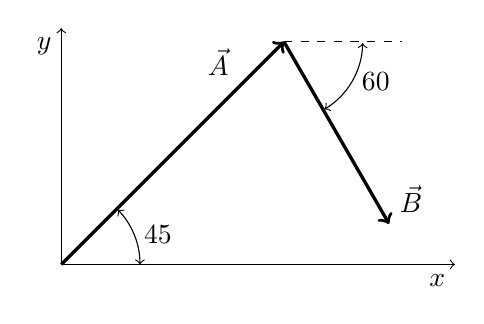
\begin{tikzpicture}
    %% Axis
    \draw[->] (0,0) -- (0,3) node[pos=1.0,anchor=north east] {$y$};
    \draw[->] (0,0) -- (5,0) node[pos=1.0,anchor=north east] {$x$};
    %% Vectors
    \draw[very thick,->] (0,0) -- (45:4) node[pos=0.8,anchor=south east] {$\vec{A}$};
    \draw[dashed] (45:4) -- ++(0:1.5);
    \draw[<->] (45:4) ++ (-59:1) arc (-59:-1:1) node[pos=0.5,anchor=west] {\ang{60}};
    \draw[<->] (0:1) arc (0:44:1) node[pos=0.5,anchor=west] {\ang{45}};
    \draw[very thick,->] (45:4) -- ++(-60:2.67) node[pos=1.0,anchor=south west] {$\vec{B}$};
\end{tikzpicture}
}

\element{halliday-mc}{
\begin{question}{halliday-ch03-q24A}
    In the diagram, $\vec{A}$ has magnitude \SI{12}{\meter} and $\vec{B}$ has magnitude \SI{8}{\meter}.
    \begin{center}
        \hallidayChThreeQTwentyFour
    \end{center}
    The $x$ component of $\vec{A}+\vec{B}$ is about:
    \begin{multicols}{3}
    \begin{choices}
        \wrongchoice{\SI{5.5}{\meter}}
        \wrongchoice{\SI{7.6}{\meter}}
      \correctchoice{\SI{12}{\meter}}
        \wrongchoice{\SI{14}{\meter}}
        \wrongchoice{\SI{15}{\meter}}
    \end{choices}
    \end{multicols}
\end{question}
}

%% NOTE: ALT: The Y component of A+B ??
%\element{halliday-mc}{
%\begin{question}{halliday-ch03-q25B}
%    In the diagram, $\vec{A}$ has magnitude \SI{12}{\meter} and $\vec{B}$ has magnitude \SI{8}{\meter}.
%    \begin{center}
%        \hallidayChThreeQTwentyFour
%    \end{center}
%    The $y$ component of $\vec{A}+\vec{B}$ is about:
%    \begin{multicols}{3}
%    \begin{choices}
%        \wrongchoice{\SI{5.5}{\meter}}
%        \wrongchoice{\SI{7.6}{\meter}}
%      \correctchoice{\SI{4.8}{\meter}}
%        \wrongchoice{\SI{14}{\meter}}
%        \wrongchoice{\SI{15}{\meter}}
%    \end{choices}
%    \end{multicols}
%\end{question}
%}


\element{halliday-mc}{
\begin{question}{halliday-ch03-q25}
    A certain vector in the $xy$ plane has an $x$ component of \SI{4}{\meter} and a $y$ component of \SI{10}{\meter}.
    It is then rotated in the $xy$ plane so its $x$ component is doubled.
    Its new $y$ component is about:
    \begin{multicols}{3}
    \begin{choices}
        \wrongchoice{\SI{20}{\meter}}
      \correctchoice{\SI{7.2}{\meter}}
        \wrongchoice{\SI{5.0}{\meter}}
        \wrongchoice{\SI{4.5}{\meter}}
        \wrongchoice{\SI{2.2}{\meter}}
    \end{choices}
    \end{multicols}
\end{question}
}

\element{halliday-mc}{
\begin{question}{halliday-ch03-q26}
    Vectors $A$ and $B$ each have magnitude $L$.
    When drawn with their tails at the same point,
        the angle between them is \ang{30}.
    The value of $\vec{A}\cdot\vec{B}$ is:
    \begin{multicols}{2}
    \begin{choices}
        \wrongchoice{zero}
        \wrongchoice{$L^2$}
      \correctchoice{$\dfrac{\sqrt{3}L^2}{2}$}
        \wrongchoice{$2L^2$}
        \wrongchoice{none of the provided}
    \end{choices}
    \end{multicols}
\end{question}
}

\element{halliday-mc}{
\begin{question}{halliday-ch03-q27}
    Let $\vec{A} = \left(\SI{2}{\meter}\right)\hat{\imath} + \left(\SI{6}{\meter}\right)\hat{\jmath} - \left(\SI{3}{\meter}\right)\hat{k}$
        and $\vec{B} = \left(\SI{4}{\meter}\right)\hat{\imath} + \left(\SI{2}{\meter}\right)\hat{\jmath} + \left(\SI{1}{\meter}\right)\hat{k}$.
    Then $\vec{A}\cdot\vec{B} = $
    \begin{choices}
        \wrongchoice{$\left(\SI{8}{\meter}\right)\hat{\imath} + \left(\SI{12}{\meter}\right)\hat{\jmath} - \left(\SI{3}{\meter}\right)\hat{k}$}
        \wrongchoice{$\left(\SI{12}{\meter}\right)\hat{\imath} - \left(\SI{14}{\meter}\right)\hat{\jmath} - \left(\SI{20}{\meter}\right)\hat{k}$}
        \wrongchoice{$\SI{23}{\meter\squared}$}
      \correctchoice{$\SI{17}{\meter\squared}$}
        \wrongchoice{none of the provided}
    \end{choices}
\end{question}
}

\element{halliday-mc}{
\begin{question}{halliday-ch03-q28}
    Two vectors have magnitudes of \SI{10}{\meter} and \SI{15}{\meter}.
    The angle between them when they are drawn with their tails at the same point is \ang{65}.
    The component of the longer vector along the line of the shorter is:
    \begin{multicols}{3}
    \begin{choices}
        \wrongchoice{zero}
        \wrongchoice{\SI{4.2}{\meter}}
      \correctchoice{\SI{6.3}{\meter}}
        \wrongchoice{\SI{9.1}{\meter}}
        \wrongchoice{\SI{14}{\meter}}
    \end{choices}
    \end{multicols}
\end{question}
}

\element{halliday-mc}{
\begin{question}{halliday-ch03-q29}
    Let $\vec{S} = \left(\SI{1}{\meter}\right)\hat{\imath} + \left(\SI{2}{\meter}\right)\hat{\jmath} + \left(\SI{2}{\meter}\right)\hat{k}$
        and $\vec{T} = \left(\SI{3}{\meter}\right)\hat{\imath} + \left(\SI{4}{\meter}\right)\hat{k}$.
    The angle between these two vectors is given by:
    \begin{multicols}{2}
    \begin{choices}
        \wrongchoice{$\cos^{-1}\left(\dfrac{14}{15}\right)$}
        \wrongchoice{$\cos^{-1}\left(\dfrac{11}{225}\right)$}
        \wrongchoice{$\cos^{-1}\left(\dfrac{104}{225}\right)$}
      \correctchoice{$\cos^{-1}\left(\dfrac{11}{15}\right)$}
        \wrongchoice{cannot be found since $\vec{S}$ and $\vec{T}$ do not lie in the same plane}
    \end{choices}
    \end{multicols}
\end{question}
}

\element{halliday-mc}{
\begin{question}{halliday-ch03-q30}
    Two vectors lie with their tails at the same point.
    When the angle between them is increased by \ang{20} their scalar product has the same magnitude but changes from positive to negative.
    The original angle between them was:
    \begin{multicols}{3}
    \begin{choices}
        \wrongchoice{\ang{0}}
        \wrongchoice{\ang{60}}
        \wrongchoice{\ang{70}}
      \correctchoice{\ang{80}}
        \wrongchoice{\ang{90}}
    \end{choices}
    \end{multicols}
\end{question}
}

\element{halliday-mc}{
\begin{question}{halliday-ch03-q31}
    If the magnitude of the sum of two vectors is less than the magnitude of either vector,
        then:
    \begin{choices}
      \correctchoice{the scalar product of the vectors must be negative}
        \wrongchoice{the scalar product of the vectors must be positive}
        \wrongchoice{the vectors must be parallel and in opposite directions}
        \wrongchoice{the vectors must be parallel and in the same direction}
        \wrongchoice{none of the provided}
    \end{choices}
\end{question}
}

\element{halliday-mc}{
\begin{question}{halliday-ch03-q32}
    If the magnitude of the sum of two vectors is greater than the magnitude of either vector,
        then:
    \begin{choices}
        \wrongchoice{the scalar product of the vectors must be negative}
        \wrongchoice{the scalar product of the vectors must be positive}
        \wrongchoice{the vectors must be parallel and in opposite directions}
        \wrongchoice{the vectors must be parallel and in the same direction}
      \correctchoice{none of the provided}
    \end{choices}
\end{question}
}

\element{halliday-mc}{
\begin{question}{halliday-ch03-q33}
    Vectors $\vec{A}$ and $\vec{B}$ each have magnitude $L$.
    When drawn with their tails at the same point,
        the angle between them is \ang{60}.
    The magnitude of the vector product $\vec{A}\times{}\vec{B}$ is:
    \begin{multicols}{2}
    \begin{choices}
        \wrongchoice{$\dfrac{L^2}{2}$}
        \wrongchoice{$L^2$}
      \correctchoice{$\dfrac{\sqrt{3}L^2}{2}$}
        \wrongchoice{$2L^2$}
        \wrongchoice{none of the provided}
    \end{choices}
    \end{multicols}
\end{question}
}

\element{halliday-mc}{
\begin{question}{halliday-ch03-q34}
    Two vectors lie with their tails at the same point.
    When the angle between them is increased by \ang{20} the magnitude of their vector product doubles.
    The original angle between them was about:
    \begin{multicols}{3}
    \begin{choices}
        \wrongchoice{\ang{0}}
      \correctchoice{\ang{18}}
        \wrongchoice{\ang{25}}
        \wrongchoice{\ang{45}}
        \wrongchoice{\ang{90}}
    \end{choices}
    \end{multicols}
\end{question}
}

\element{halliday-mc}{
\begin{question}{halliday-ch03-q35}
    Two vectors have magnitudes of \SI{10}{\meter} and \SI{15}{\meter}.
    The angle between them when they are drawn with their tails at the same point is \ang{65}.
    The component of the longer vector along the line perpendicular to the shorter vector,
        in the plane of the vectors, is:
    \begin{multicols}{3}
    \begin{choices}
        \wrongchoice{zero}
        \wrongchoice{\SI{4.2}{\meter}}
        \wrongchoice{\SI{6.3}{\meter}}
        \wrongchoice{\SI{9.1}{\meter}}
      \correctchoice{\SI{14}{\meter}}
    \end{choices}
    \end{multicols}
\end{question}
}

\element{halliday-mc}{
\begin{question}{halliday-ch03-q36}
    The two vectors $\left(\SI{3}{\meter}\right)\hat{\imath} - \left(\SI{2}{\meter}\right)\hat{\jmath}$
        and $\left(\SI{2}{\meter}\right)\hat{\imath} + \left(\SI{3}{\meter}\right)\hat{\jmath} - \left(\SI{2}{\meter}\right)\hat{k}$ define a plane.
    It is the plane of the triangle with both tails at one vertex and each head at one of the other vertices.
    Which of the following vectors is perpendicular to the plane?
    \begin{choices}
      \correctchoice{$\left(\SI{4}{\meter}\right)\hat{\imath} + \left(\SI{6}{\meter}\right)\hat{\jmath} + \left(1\SI{3}{\meter}\right)\hat{k}$}
        \wrongchoice{$\left(\SI{-4}{\meter}\right)\hat{\imath} + \left(\SI{6}{\meter}\right)\hat{\jmath} + \left(1\SI{3}{\meter}\right)\hat{k}$}
        \wrongchoice{$\left(\SI{4}{\meter}\right)\hat{\imath} - \left(\SI{6}{\meter}\right)\hat{\jmath} + \left(1\SI{3}{\meter}\right)\hat{k}$}
        \wrongchoice{$\left(\SI{4}{\meter}\right)\hat{\imath} + \left(\SI{6}{\meter}\right)\hat{\jmath} - \left(1\SI{3}{\meter}\right)\hat{k}$}
        \wrongchoice{$\left(\SI{4}{\meter}\right)\hat{\imath} + \left(\SI{6}{\meter}\right)\hat{\jmath}$}
    \end{choices}
\end{question}
}

\element{halliday-mc}{
\begin{question}{halliday-ch03-q37}
    Let $\vec{R} = \vec{S}\times\vec{T}$ and $\theta=\ang{90}$,
        where $\theta$ is the angle between $\vec{S}$ and $\vec{T}$
        when they are drawn with their tails at the same point.
    Which of the following is \emph{not} true?
    \begin{multicols}{2}
    \begin{choices}
        \wrongchoice{$\left|\vec{R}\right| = \left|\vec{S}\right| \left|\vec{T}\right|\sin\theta$}
        \wrongchoice{$-\vec{R} = \vec{T}\times\vec{S}$}
        \wrongchoice{$\vec{R}\cdot{}\vec{S} = 0$}
        \wrongchoice{$\vec{R}\cdot{}\vec{T} = 0$}
      \correctchoice{$\vec{S}\cdot{}\vec{T} = 0$}
    \end{choices}
    \end{multicols}
\end{question}
}

\element{halliday-mc}{
\begin{question}{halliday-ch03-q38}
    The value of $\hat{\imath}\cdot\left(\hat{\jmath}\times\hat{k}\right)$ is:
    \begin{multicols}{3}
    \begin{choices}
        \wrongchoice{zero}
      \correctchoice{$+1$}
        \wrongchoice{$-1$}
        \wrongchoice{$3$}
        \wrongchoice{$\sqrt{3}$}
    \end{choices}
    \end{multicols}
\end{question}
}

\element{halliday-mc}{
\begin{question}{halliday-ch03-q39}
    The value of $\hat{k}\cdot\left(\hat{k}\times\hat{\imath}\right)$ is:
    \begin{multicols}{3}
    \begin{choices}
      \correctchoice{zero}
        \wrongchoice{$+1$}
        \wrongchoice{$-1$}
        \wrongchoice{$3$}
        \wrongchoice{$\sqrt{3}$}
    \end{choices}
    \end{multicols}
\end{question}
}


\endinput


